\documentclass[journal,twoside,web]{ieeecolor}
\usepackage{jsen}
\usepackage{cite}
\usepackage{amsmath,amssymb,amsfonts}
\usepackage{graphicx}
\usepackage{textcomp}
\usepackage{array}
\usepackage{url}
\newcolumntype{L}[1]{>{\raggedright\arraybackslash}p{#1}}
\setlength{\tabcolsep}{3pt}
\sloppy
\def\BibTeX{{\rm B\kern-.05em{\sc i\kern-.025em b}\kern-.08em
    T\kern-.1667em\lower.7ex\hbox{E}\kern-.125emX}}

\markboth{Spring 2026}
{Diver: Machine Learning Pipeline Using GitHub Actions}

\begin{document}

\title{Machine Learning Pipeline Using GitHub Actions: Metro Traffic Volume Classifier}

\author{Lorc\'an Diver, MSc. Big Data Analytics and AI
\thanks{Under the supervision of Dr. Shagufta Henna, Atlantic Technological University. Public repository link is included in the report body.}}

\IEEEtitleabstractindextext{%
\begin{abstract}
This report describes a working MLOps artefact built around the public UCI Metro Interstate Traffic Volume dataset. The model predicts whether an hourly traffic record represents normal traffic or high traffic using weather, calendar, holiday and lagged traffic features. The main aim was not only to train a classifier, but to build a repeatable machine learning pipeline that can be rerun, checked, served, containerised, deployed and monitored. The artefact uses GitHub Actions for continuous integration, data preprocessing, model training and evaluation, Docker image checks, Kind Kubernetes deployment, continuous training, continuous monitoring, security checks and final readiness evidence. The trained scikit-learn pipeline is served through a Flask API and browser UI. Docker packages the API and saved model, while Kind Kubernetes shows that the container can run behind a Kubernetes service and pass health and prediction smoke tests. The current model version is 1.0.1, with accuracy 0.979, macro F1 0.979, weighted F1 0.979 and ROC AUC 0.998 on the held-out test set. A strict quality gate with a 0.975 target accepted the candidate model and would reject a weaker retrained model. Screenshots, command logs and report files under \texttt{reports/} provide external-examiner evidence that the artefact works end to end.
\end{abstract}

\begin{IEEEkeywords}
MLOps, GitHub Actions, Continuous Integration, Continuous Delivery, Continuous Training, Continuous Monitoring, Flask API, Docker, Kind Kubernetes, model registry, drift check.
\end{IEEEkeywords}}

\maketitle

\section{Introduction}
\IEEEPARstart{T}{his} project is a machine learning pipeline for classifying traffic-volume records from the UCI Metro Interstate Traffic Volume dataset. The target variable is \texttt{high\_traffic}, a binary label derived from the original \texttt{traffic\_volume} column. A record is labelled high traffic when the hourly traffic count is at least 3800; otherwise it is labelled normal traffic. The model uses 15 features: weather measurements, calendar fields, weekend and holiday flags, the \texttt{weather\_main} category, lagged traffic volumes and rolling traffic averages.

The report is a supporting document for the artefact, not a replacement for it. The working evidence is in the public GitHub repository: \url{https://github.com/lorcan973232/mlops-metro-traffic-volume-pipeline}. The repository contains the source code, tests, workflows, Dockerfile, Kind manifests, saved model, metrics, monitoring outputs, screenshots and command logs. MLOps in this project means that the model is treated as part of a controlled software system: data preparation, training, evaluation, serving, deployment, monitoring and retraining are all scripted and checked.

GitHub Actions was chosen because the assessment requires a machine learning pipeline using workflow automation. It also gives a visible audit trail for an external examiner. The workflows show which command ran, when it ran, whether it passed, and which artefacts were uploaded. This matters because a model score alone does not prove that an ML system can be rerun or deployed.

\section{Use Case and Dataset}
The use case is short-horizon traffic triage. Given weather, time and recent traffic signals, the system predicts whether an hourly record is likely to be high traffic. This is suitable for a student MLOps project because the dataset is public, has enough rows for train/test evaluation, includes a realistic mix of numerical and categorical features, and can be processed without relying on private data or manual data collection.

Only one dataset is used: the UCI Metro Interstate Traffic Volume dataset by Hogue \cite{uci}. The raw file is stored as \path{data/raw/Metro_Interstate_Traffic_Volume.csv.gz}; the processed file is \path{data/processed/metro-traffic-processed.csv}. The ingestion report records the official source and raw SHA-256 hash. The preprocessing step derives the binary target and creates lag features from previous traffic records only. The current traffic-volume value is not used directly as a feature, which reduces target leakage.

\begin{table}[!t]
\caption{Main build decisions}
\label{tab:approach}
\centering
\scriptsize
\renewcommand{\arraystretch}{1.12}
\begin{tabular}{|L{0.62in}|L{1.05in}|L{0.95in}|}
\hline
\textbf{Area} & \textbf{Choice} & \textbf{Reason} \\
\hline
Dataset & UCI Metro Interstate Traffic Volume & Public, repeatable and suitable for traffic classification. \\
\hline
Model & scikit-learn hist-gradient boosting pipeline & Strong tabular classifier with inspectable preprocessing. \\
\hline
API & Flask health and prediction routes & Simple serving layer with schema checks and browser UI. \\
\hline
Deploy & Docker plus Kind & Proves packaging and Kubernetes rollout locally. \\
\hline
Automation & GitHub Actions & Gives CI/CD/CT/CM evidence per commit or schedule. \\
\hline
\end{tabular}
\end{table}

\section{Academic Justification}
Sculley et al. argue that machine learning systems can build hidden technical debt when data dependencies, configuration, tests and serving code are not controlled together \cite{sculley}. This artefact responds to that risk by making the data, training, evaluation, API, Docker and Kubernetes paths explicit and repeatable. Amershi et al. show that ML software needs engineering practices around data management, model development and deployment, rather than isolated notebooks \cite{amershi}. The repository therefore uses scripts, tests and workflows instead of manual model training.

The quality gate follows the production-readiness argument in Breck et al. \cite{breck}. A retrained candidate is not automatically accepted; it must meet threshold checks and provide required reports. Monitoring and drift checks are also included because Gama et al. show that data streams can change over time \cite{gama}. In this project, monitoring is deliberately lightweight and honest: offline reports check schema, missing values, feature summaries and Population Stability Index (PSI) drift; API-aware mode checks a live URL when one is supplied.

Containerisation and Kubernetes are justified by reproducibility and deployment control. Docker packages the Flask application, dependencies and saved model in one image \cite{docker}. Kubernetes and Kind provide a local cluster path for applying deployments, exposing a service and checking rollout status \cite{kubernetes,kind}. GitHub Actions provides the automation layer for continuous integration and delivery \cite{githubactions}.

\section{Artefact Construction}
The artefact was built as a sequence of controlled stages. First, the repository structure was created with separate folders for \texttt{src/}, \texttt{app/}, \texttt{tests/}, \texttt{deployment/}, \texttt{models/} and \texttt{reports/}. Data ingestion validates the public dataset and records source metadata. Preprocessing derives the classification target, creates lag and rolling features, and saves a deterministic processed CSV. Model selection compares candidate settings before final training. Training saves the model bundle, while evaluation writes metrics, a classification report, confusion matrices, cross-validation results and the quality-gate report.

The serving layer is a Flask API in \texttt{app/main.py}. The \texttt{/health} route confirms model loading, dataset metadata, schema and model version. The \texttt{/predict} route validates input features and returns prediction labels, probabilities and confidence. A browser UI calls the real \texttt{/predict} route, so the demo is not a mock. Tests cover data validation, preprocessing, model pipeline contracts, API behaviour, UI schema, monitoring reports, workflow files and artefact evidence.

\begin{table*}[!t]
\caption{MLOps artefact stages and evidence}
\label{tab:stages}
\centering
\scriptsize
\renewcommand{\arraystretch}{1.13}
\begin{tabular}{|L{0.72in}|L{1.25in}|L{1.45in}|L{3.0in}|}
\hline
\textbf{Stage} & \textbf{What was created} & \textbf{Main files} & \textbf{Why it matters} \\
\hline
Repository setup & Public repo, README, evidence folders & \texttt{README.md}, \texttt{reports/} & Gives a repeatable route for local run, review and external marking. \\
\hline
Ingestion & Raw public data check and source report & \texttt{src/data.py}, \texttt{data\_ingestion.json} & Shows the dataset source, raw file hash, schema and target definition. \\
\hline
Preprocessing & Deterministic training table & \texttt{src/preprocess.py}, processed CSV & Creates target, lag features and rolling features without using current target as input. \\
\hline
Selection & Candidate model and final model bundle & \texttt{src/model\_selection.py}, \texttt{src/train.py}, \texttt{models/} & Separates candidate comparison from final model saving. \\
\hline
Registry & Metrics, gate and active version & \texttt{src/evaluate.py}, \texttt{src/model\_registry.py} & Makes model acceptance explicit and records version 1.0.1. \\
\hline
API/UI & Flask health, predict and browser demo & \texttt{app/} & Proves the saved model can be used outside the training script. \\
\hline
Testing & 36 current passing tests & \texttt{tests/} & Checks data, model, API, UI, monitoring, workflows and report evidence. \\
\hline
Docker/Kind & Container and local Kubernetes deployment & \texttt{Dockerfile}, \texttt{deployment/kind/} & Shows the API can run in a packaged and orchestrated environment. \\
\hline
CT/CM & Scheduled retraining, monitoring and scans & \texttt{.github/workflows/} & Provides later-stage MLOps evidence beyond basic CI. \\
\hline
\end{tabular}
\end{table*}

\section{Branching Strategy}
The repository uses a simple branch strategy that fits a student MLOps artefact. The \texttt{main} branch is the stable submission branch. A \texttt{develop} branch is used as an integration branch before changes move to \texttt{main}. Feature branches are used for new work, then merged by pull request. Pull requests and pushes trigger CI checks. Pushes to \texttt{main} also trigger deployment and readiness workflows. Scheduled workflows handle continuous training and continuous monitoring.

This is appropriate because the project has one maintainer and a fixed assessment scope. More complex release branching would add process without adding useful evidence. The saved branching report in \texttt{reports/submission/branching\_evidence.md} records merged feature-to-develop and develop-to-main pull requests and the checks attached to them.

\section{GitHub Actions Pipeline}
The GitHub Actions workflows are the core MLOps evidence. They implement at least five pipeline stages from the brief: data acquisition/preprocessing, model training/testing, model deployment, continuous integration, continuous delivery, continuous training and continuous monitoring.

\begin{table*}[!t]
\caption{Workflow detail}
\label{tab:workflows}
\centering
\scriptsize
\renewcommand{\arraystretch}{1.12}
\begin{tabular}{|L{1.05in}|L{0.85in}|L{2.15in}|L{2.35in}|}
\hline
\textbf{Workflow/file} & \textbf{Trigger} & \textbf{What it runs} & \textbf{Evidence and failure condition} \\
\hline
CI / \texttt{ci.yml} & push, PR, manual & install, Ruff, stale-evidence scan, compile, pytest, ML smoke path, monitoring scripts & uploads CI artefacts; fails on lint, tests, model rejection or script errors. \\
\hline
Data preprocessing / \texttt{data-preprocessing.yml} & data/code changes, PR, manual & \texttt{src.data}, \texttt{src.preprocess}, processed CSV check & uploads ingestion and preprocessing artefacts; fails if data, schema or output is missing. \\
\hline
Train and evaluate / \texttt{train-and-evaluate.yml} & source/test changes, PR, manual & data, preprocessing, selection, train, evaluate, registry, prediction, explainability, fairness, cost-benefit & uploads model and reports; fails on missing required reports or a rejected model. \\
\hline
Docker build / \texttt{docker-build.yml} & push, PR, manual & build image, run container on port 5001, health check, prediction smoke test, latency benchmark & uploads Docker logs; fails if image build or API smoke test fails. \\
\hline
Deploy Kind / \texttt{deploy.yml} & main push, manual, after Docker & build image, create Kind, load image, apply manifests, rollout status, port-forward, smoke test & uploads Kind logs; fails if rollout or API smoke test fails. \\
\hline
Continuous Training / \texttt{continuous-training.yml} & weekly, manual & retrains candidate, evaluates, runs explainability/fairness/cost reports, enforces quality-gate contract & uploads CT candidate and gate; rejects weaker or incomplete candidates. \\
\hline
Monitoring / \texttt{monitoring.yml} & daily, manual & rebuilds metadata, runs data-quality checks, PSI drift check and retraining flags & uploads monitoring reports; fails if required monitoring/drift fields are missing. \\
\hline
Security/readiness / \texttt{security-scan.yml}, \texttt{final-readiness.yml} & push, PR or main & secret scan, dependency scan, Docker non-root check, SBOM, compile, tests, lint, visibility check & uploads security and readiness reports; fails on unsafe runtime, stale evidence or visibility problems. \\
\hline
\end{tabular}
\end{table*}

Continuous Training is more than a scheduled retrain. It creates a candidate model and then runs a separate quality-gate job. That job checks that required metrics and reports exist, that explainability and fairness reports were computed, and that the saved quality gate passed. Only after this does the promote job register the accepted candidate. Continuous Monitoring is also explicit: it prepares model metadata, checks the processed batch, runs the drift script and uploads data-quality and drift reports.

\section{Deployment Architecture}
The deployment path is:
\begin{center}
\scriptsize Data $\rightarrow$ Preprocess $\rightarrow$ Train $\rightarrow$ Evaluate $\rightarrow$ Saved model\\
$\rightarrow$ Flask API $\rightarrow$ Docker $\rightarrow$ Kind Kubernetes $\rightarrow$ Smoke test
\end{center}
The Flask application loads \path{models/traffic_volume_classifier.joblib}. Docker builds an image containing the application, requirements and saved model. Kind creates a local Kubernetes cluster, loads the Docker image, applies the deployment and service YAML, waits for rollout, then uses port-forwarding to expose the service on \texttt{127.0.0.1:8080}. Smoke tests call \texttt{/health} and \texttt{/predict}. Current local checks passed for Flask on port 5000, Docker on port 5001 and the Kind port-forward on port 8080. A fresh \texttt{kubectl get pods} command was blocked by a local cluster connection reset in the current shell, so the report relies on saved Kind logs/screenshots plus the live 8080 smoke-test response for current evidence.

\section{Evaluation and Quality Gates}
The current accepted model is version 1.0.1. It uses \texttt{HistGradientBoostingClassifier} with balanced class weighting, learning rate 0.06, 320 iterations and 31 leaf nodes. Selection used stratified cross-validation and macro F1 as the main scoring metric. The final test set was held back until final evaluation.

\begin{table}[!t]
\caption{Current model quality evidence}
\label{tab:metrics}
\centering
\scriptsize
\renewcommand{\arraystretch}{1.12}
\begin{tabular}{|L{1.05in}|L{0.5in}|L{0.92in}|}
\hline
\textbf{Metric/check} & \textbf{Value} & \textbf{Evidence} \\
\hline
Accuracy & 0.979 & metrics JSON \\
\hline
Balanced accuracy & 0.978 & metrics JSON \\
\hline
Macro F1 & 0.979 & metrics JSON \\
\hline
Weighted F1 & 0.979 & metrics JSON \\
\hline
ROC AUC & 0.998 & metrics JSON \\
\hline
Baseline accuracy & 0.541 & baseline JSON \\
\hline
Quality target & 0.975 & gate report \\
\hline
Gate decision & accept & gate report \\
\hline
Test suite & 36 pass & \texttt{pytest -q} \\
\hline
\end{tabular}
\end{table}

The model should not be described as a final forecasting product. Its value for the assessment is that it passes a strict, reproducible acceptance route and is served through a working API. A weaker retrained model would be rejected because \texttt{src.evaluate} can fail on rejection and the CT workflow separately enforces the quality-gate contract.

\section{Working Evidence}
The report uses the most important screenshots in the main pages. Additional screenshots and command logs remain under \texttt{reports/screenshots/} and \texttt{reports/submission/command-logs/}. The screenshots show the public repository, successful Actions runs, Flask UI, prediction result, health endpoint, Kind resources and quality gate.

\begin{figure*}[!t]
\centering
\begin{minipage}{0.31\textwidth}
\centering
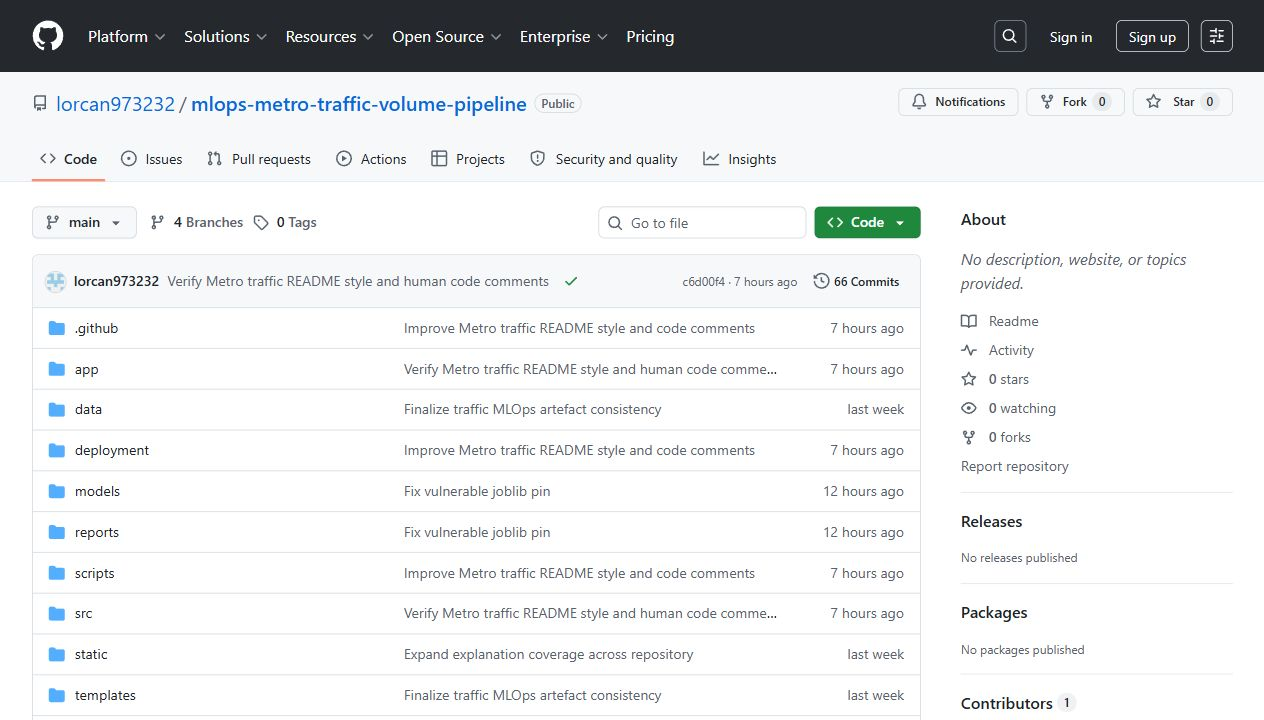
\includegraphics[width=\linewidth]{fig_github_repository.png}
{\scriptsize Public repository and project files.\par}
\end{minipage}\hfill
\begin{minipage}{0.31\textwidth}
\centering
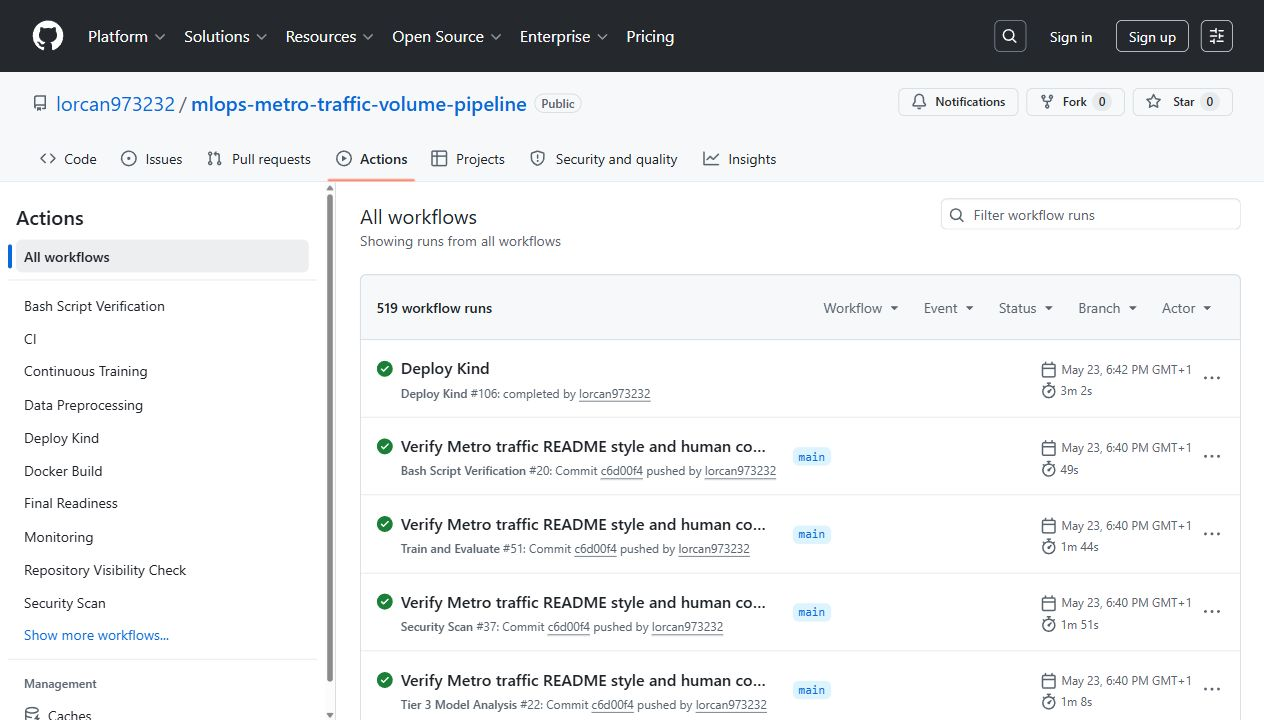
\includegraphics[width=\linewidth]{fig_github_actions.png}
{\scriptsize Successful GitHub Actions runs.\par}
\end{minipage}\hfill
\begin{minipage}{0.31\textwidth}
\centering
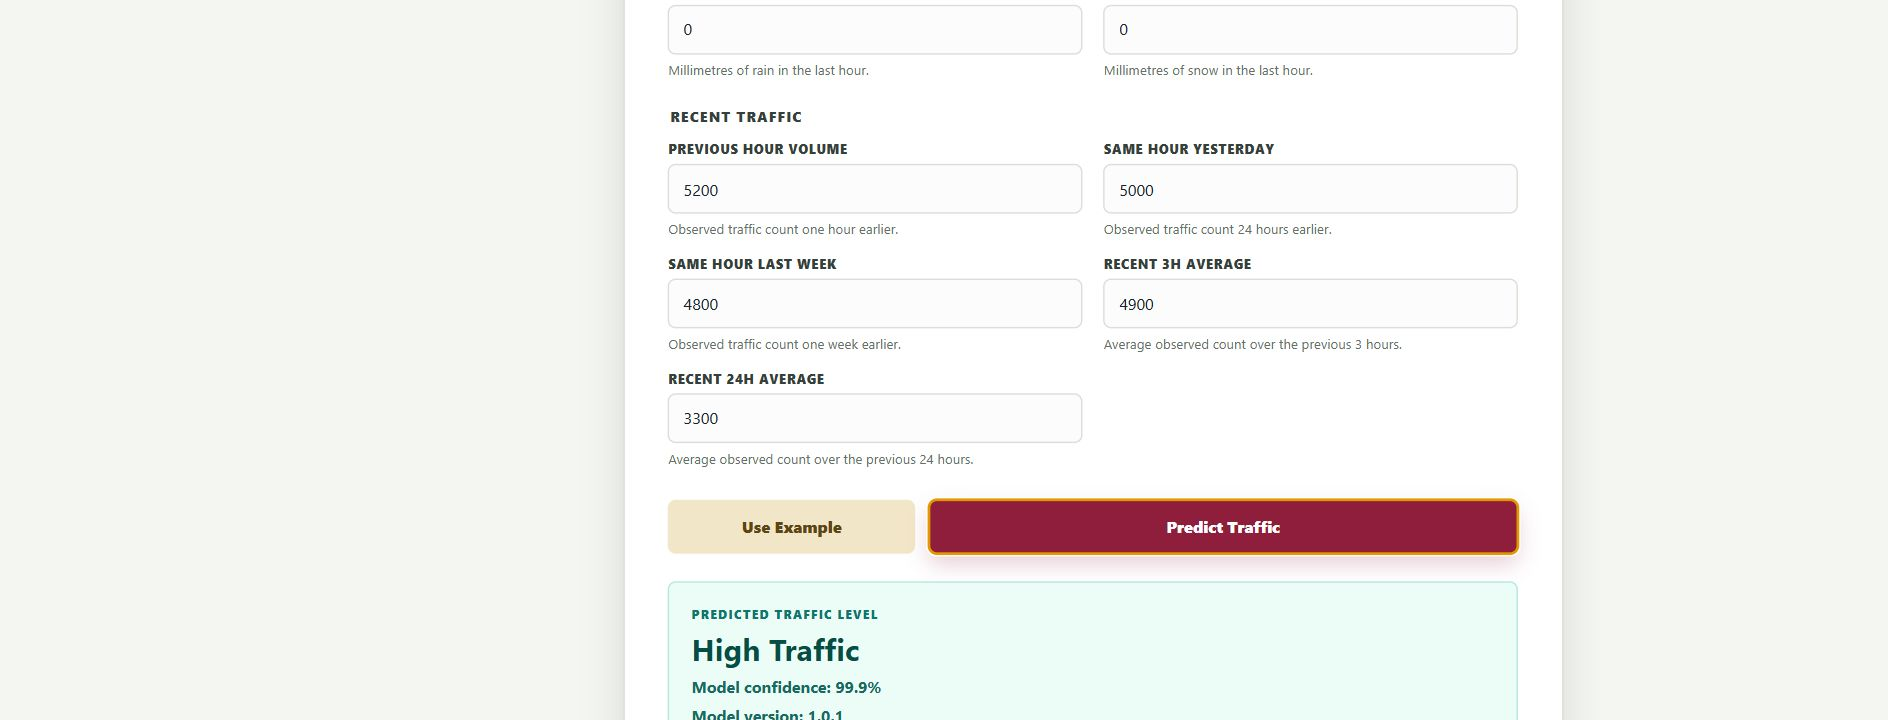
\includegraphics[width=\linewidth]{fig_flask_prediction.png}
{\scriptsize Flask UI prediction using the real API.\par}
\end{minipage}
\vspace{0.06in}
\begin{minipage}{0.31\textwidth}
\centering
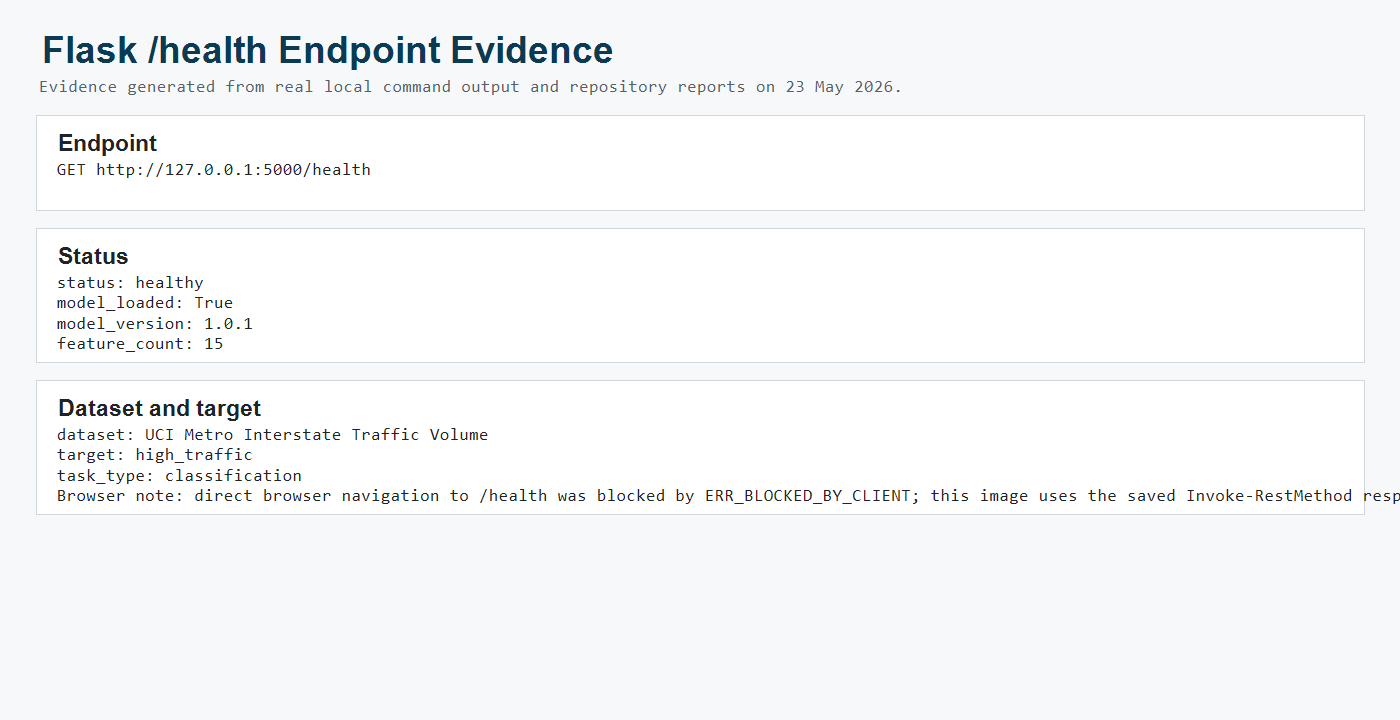
\includegraphics[width=\linewidth]{fig_health.png}
{\scriptsize Health endpoint with model metadata.\par}
\end{minipage}\hfill
\begin{minipage}{0.31\textwidth}
\centering
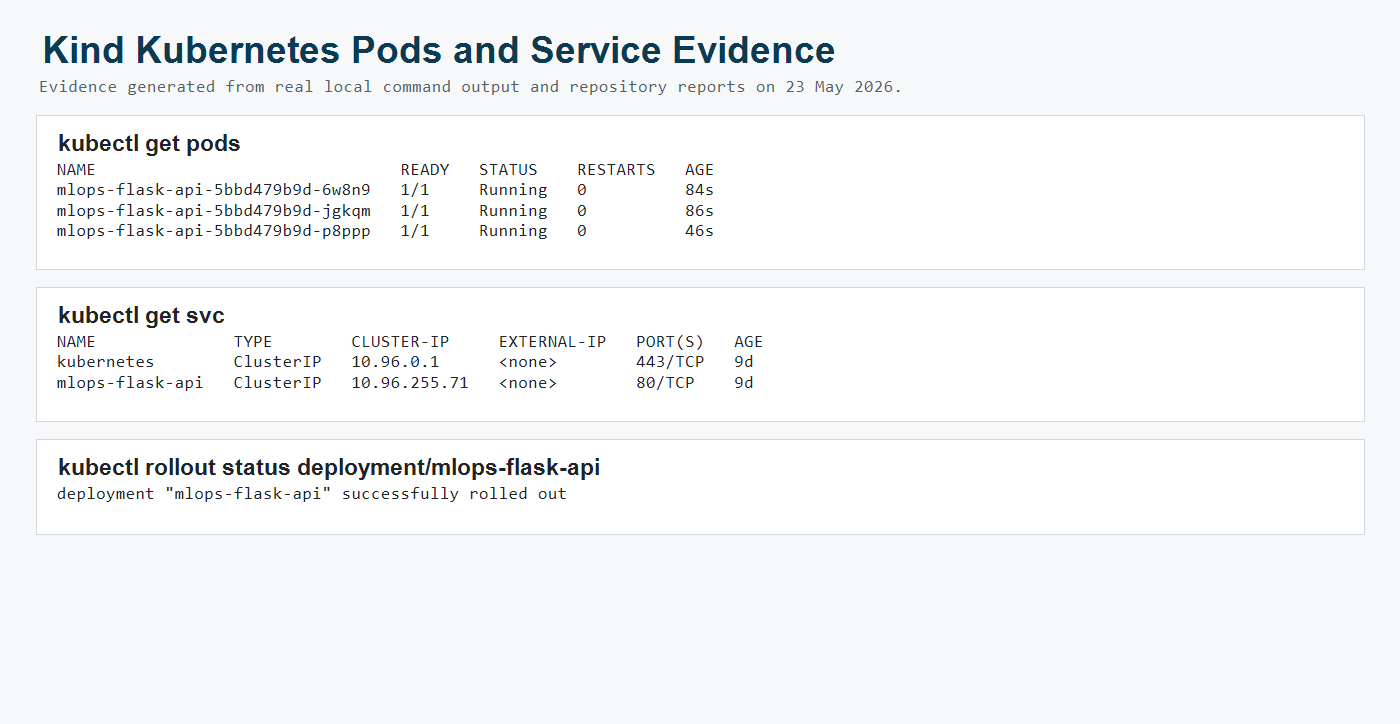
\includegraphics[width=\linewidth]{fig_kind.png}
{\scriptsize Kind pods, service and rollout evidence.\par}
\end{minipage}\hfill
\begin{minipage}{0.31\textwidth}
\centering
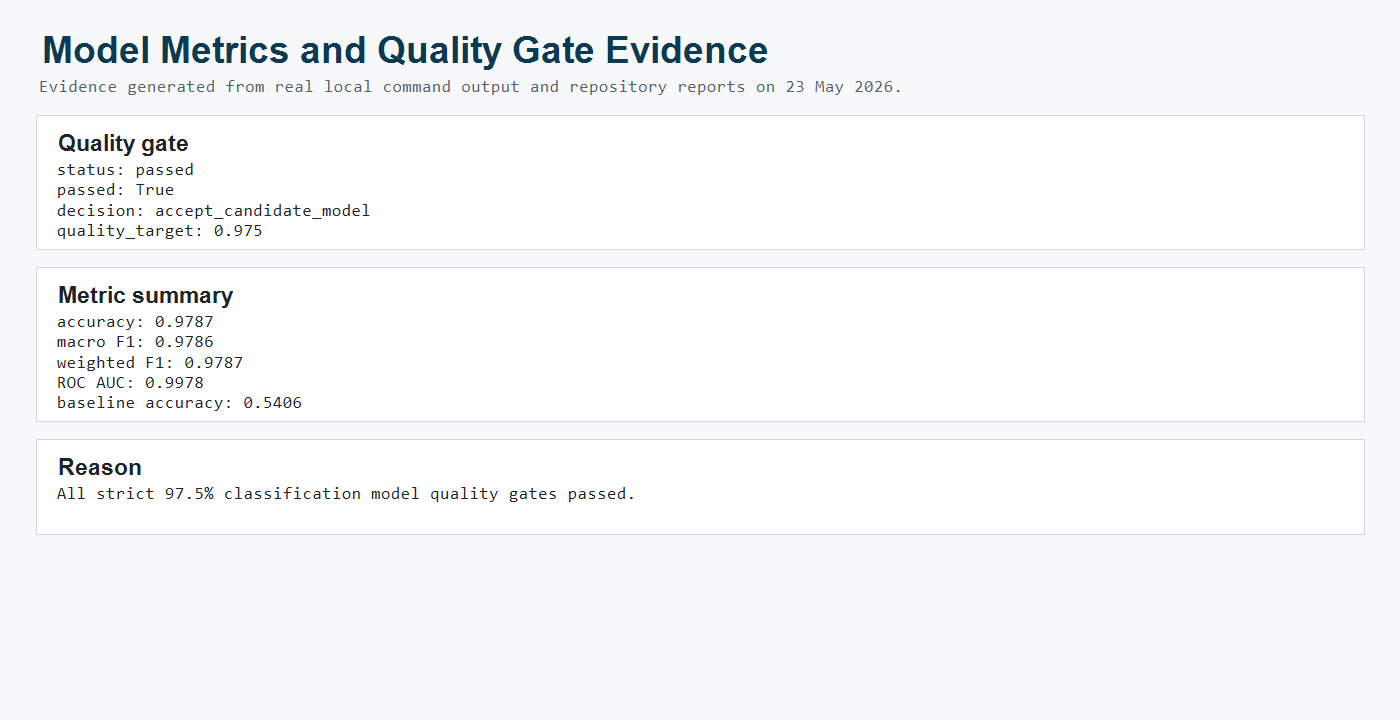
\includegraphics[width=\linewidth]{fig_quality_gate.png}
{\scriptsize Quality gate and model metrics evidence.\par}
\end{minipage}
\caption{Working evidence screenshots used in the report. The full-resolution files are stored in \texttt{reports/screenshots/}.}
\label{fig:evidence}
\end{figure*}

\section{Limitations and Discussion}
The artefact is a student MLOps project, not a live traffic-control service. Monitoring is lightweight and simulated unless API-aware mode is run against a live URL. Kind is a local Kubernetes environment, not a permanent public cloud service. The fairness check uses non-sensitive traffic and weather proxy groups because the dataset has no demographic protected attributes. These limits are stated in the reports rather than hidden.

The main strength is traceability. The same repository contains the data code, training code, tests, workflows, model bundle, API, Dockerfile, Kind YAML, screenshots and generated evidence. The main weakness is that deployment is local rather than hosted continuously. However, for the assessment brief, Kind is an acceptable deployment route and is checked by workflow and local smoke tests.

\section{Conclusion}
The artefact implements the required MLOps stages using real code and real evidence. It includes data acquisition and preprocessing, model training and testing, Flask deployment, Docker containerisation, Kind Kubernetes deployment, Continuous Integration, Continuous Delivery, Continuous Training and Continuous Monitoring. GitHub Actions makes the pipeline repeatable and visible. The quality gate protects against accepting weak retrained models. Docker and Kind show that the saved model can be served outside the training environment. The screenshots and command logs prove that the demo, API, workflows and reports were checked.

\begin{thebibliography}{00}
\bibitem{sculley} D. Sculley et al., ``Hidden Technical Debt in Machine Learning Systems,'' in \textit{Advances in Neural Information Processing Systems}, 2015.
\bibitem{amershi} S. Amershi et al., ``Software Engineering for Machine Learning: A Case Study,'' in \textit{Proceedings of the 41st International Conference on Software Engineering: Software Engineering in Practice}, 2019.
\bibitem{breck} E. Breck et al., ``The ML Test Score: A Rubric for ML Production Readiness and Technical Debt Reduction,'' in \textit{IEEE Big Data}, 2017.
\bibitem{gama} J. Gama, I. Zliobaite, A. Bifet, M. Pechenizkiy and A. Bouchachia, ``A Survey on Concept Drift Adaptation,'' \textit{ACM Computing Surveys}, vol. 46, no. 4, 2014.
\bibitem{uci} J. Hogue, ``Metro Interstate Traffic Volume,'' UCI Machine Learning Repository, DOI: 10.24432/C5X60B, 2019.
\bibitem{docker} Docker Inc., ``Docker overview,'' Docker Docs, 2026. Available: \url{https://docs.docker.com/get-started/docker-overview/}
\bibitem{kubernetes} Kubernetes, ``Deployments'' and ``Services,'' Kubernetes Documentation, 2026. Available: \url{https://kubernetes.io/docs/}
\bibitem{kind} Kubernetes SIGs, ``kind: Kubernetes in Docker,'' 2026. Available: \url{https://kind.sigs.k8s.io/}
\bibitem{githubactions} GitHub, ``GitHub Actions documentation,'' 2026. Available: \url{https://docs.github.com/actions}
\end{thebibliography}

\end{document}
